\subsection{弱解}\label{sec:conservation-weak-solutions}

如上一节所见, 双曲守恒律的光滑解可在有限时间内爆破 (产生间断或奇性). 但这并非仅仅是数学上的奇特现象. 早在十九世纪, 人们就观察到某些物理波动本质上是不连续的, 线性波动方程无法预言这些现象. 在这种情形下, 不能沿用即使微分方程本身已无意义仍接受其解的做法 (在波动方程的 D'Alembert 解中曾可这样做), 因为非线性问题的闭式解无法算出. 为了理解 (并计算) 不连续解, 需要推广解本身的概念.

\begin{Definition}
\label{def:conservation-weak-solution}
方程 \eqref{eq:conservation-law-system}, \eqref{eq:conservation-law-cauchy-data} 的\textbf{弱解}是函数 $\bm{u}:\mathbb{R}^{2+}\to\mathbb{R}^n$, 它对每个 $\bm{\phi}\in C_0^1(\mathbb{R}^{2+})$ 满足
\begin{equation}\label{eq:conservation-weak-solution}
\begin{aligned}
&\int_0^\infty\int_{-\infty}^\infty[\bm{u}(x,t)\cdot\bm{\phi}_t(x,t)+\bm{f}(\bm{u}(x,t))\cdot\bm{\phi}_x(x,t)]\,\mathrm{d}x\,\mathrm{d}t\\
&\qquad+\int_{-\infty}^\infty\bm{u}_0(x)\bm{\phi}(x,0)\,\mathrm{d}x=0
\end{aligned}
\end{equation}
这里
\begin{equation}\label{eq:conservation-test-function-space}
C_0^1(\mathbb{R}^{2+}):=\{\bm{\phi}\in C^1(\mathbb{R}^{2+})\mid\exists r>0\text{ s.t. }\operatorname{supp}\bm{\phi}\subset B_r((0,0))\cap\mathbb{R}^{2+}\}.
\end{equation}

\end{Definition}

首先指出, 这一定义确实是经典解概念的推广, 由此开始对弱解的研究.

\begin{Theorem}
\label{thm:classical-conservation-solutions-weak}
假设 $\bm{u}\in C^1(\mathbb{R}^{2+})$ 是 \eqref{eq:conservation-law-system}, \eqref{eq:conservation-law-cauchy-data} 的经典解. 那么 $\bm{u}$ 也是弱解.
\end{Theorem}

\begin{Proof}
证明只是平面上 Green 定理的一个简单应用. 任取 $\bm{\phi}\in C_0^1(\mathbb{R}^{2+})$, 并将 $r$ 取得足够大, 使 $\operatorname{supp}\bm{\phi}\subseteq S$, 其中 $S=B_r((0,0))\cap\mathbb{R}^{2+}$. 注意, 由于 $\bm{u}$ 在经典意义下满足 \eqref{eq:conservation-law-system}, 有
\begin{equation}\label{eq:conservation-classical-product-identity}
(\bm{u}\cdot\bm{\phi})_t+(\bm{f}(\bm{u})\cdot\bm{\phi})_x=\bm{u}\cdot\bm{\phi}_t+\bm{f}(\bm{u})\cdot\bm{\phi}_x.
\end{equation}
因此, 结合 Green 定理及关于 $\bm{\phi}$ 支集的信息, 得到
\[
\begin{aligned}
&\int\!\!\int_{\mathbb{R}^{2+}}\bm{u}\cdot\bm{\phi}_t+\bm{f}(\bm{u})\cdot\bm{\phi}_x\,\mathrm{d}x\,\mathrm{d}t\\
&=\int\!\!\int_S(\bm{u}\cdot\bm{\phi})_t+(\bm{f}(\bm{u})\cdot\bm{\phi})_x\,\mathrm{d}x\,\mathrm{d}t\\
&=-\int_{\partial S}\bm{u}\cdot\bm{\phi}\,\mathrm{d}x-\bm{f}(\bm{u})\cdot\bm{\phi}\,\mathrm{d}t\\
&=-\int_{-\infty}^\infty\bm{u}(x,0)\cdot\bm{\phi}(x,0)\,\mathrm{d}x\\
&=-\int_{-\infty}^\infty\bm{u}_0(x)\cdot\bm{\phi}(x,0)\,\mathrm{d}x.
\end{aligned}
\]
这里倒数第二个等式源于在半圆 $t=(r^2-x^2)^{1/2}$ 上 $\bm{\phi}=0$. 最后一个等式源于 $\bm{u}$ 满足初始条件 \eqref{eq:conservation-law-cauchy-data}.
\end{Proof}

\subsubsection{Rankine-Hugoniot 条件}\label{subsec:rankine-hugoniot-condition}

既然已定义弱解, 现在来寻找不连续弱解的必要条件.

以下分片光滑弱解的必要条件 \eqref{eq:rankine-hugoniot-jump-condition} 称为 Rankine-Hugoniot 条件.

\begin{Theorem}{Rankine-Hugoniot}
\label{thm:rankine-hugoniot}
设 $N$ 为开上半平面中的一个开邻域, 曲线 $C:(\alpha,\beta)\ni t\mapsto\hat x(t)$ 将 $N$ 分成两部分 $N^l$ 和 $N^r$, 分别位于曲线的左侧与右侧. 设 $\bm{u}$ 是 \eqref{eq:conservation-law-system} 的弱解 (这里初始条件无关紧要), 且满足
\begin{enumerate}
\item $\bm{u}$ 在 $N^l$ 和 $N^r$ 中都是 \eqref{eq:conservation-law-system} 的经典解,
\item $\bm{u}$ 在曲线 $C$ 处发生跳跃间断 $[\bm{u}]$, 并且
\item 跳跃 $[\bm{u}]$ 沿 $C$ 连续.
\end{enumerate}
对任意 $\bm{p}\in C$, 令 $s:=\hat x'(\bm{p})$ 为 $C$ 在 $\bm{p}$ 处的斜率. 那么曲线与跳跃之间成立以下关系:
\begin{equation}\label{eq:rankine-hugoniot-jump-condition}
s[\bm{u}]=[\bm{f}(\bm{u})].
\end{equation}
这里对任意 $\bm{p}=(x_0,t_0)\in C$, 定义
\begin{equation}\label{eq:conservation-jump-definition}
\begin{aligned}
[\bm{u}](\bm{p})&:=\bm{u}^r(\bm{p})-\bm{u}^l(\bm{p})\\
&:=\lim_{(x^r,t^r)\xrightarrow{r}\bm{p}}\bm{u}(x^r,t^r)-\lim_{(x^l,t^l)\xrightarrow{l}\bm{p}}\bm{u}(x^l,t^l)
\end{aligned}
\end{equation}
其中符号 $\xrightarrow{r}\bm{p}$ 表示点 $(x^r,t^r)\in N^r$ 趋于 $\bm{p}$ 的极限, $\xrightarrow{l}\bm{p}$ 表示点 $(x^l,t^l)\in N^l$ 趋于 $\bm{p}$ 的极限.
\end{Theorem}

\begin{Proof}
令 $\bm{\phi}\in C_0^1(\mathbb{R}^{2+})$ 为任意支集位于 $N$ 中的检验函数. 由于 $\bm{u}$ 是弱解, 可写为
\[
\begin{aligned}
0&=\int_N\bm{u}\cdot\bm{\phi}_t+\bm{f}(\bm{u})\cdot\bm{\phi}_x\,\mathrm{d}x\,\mathrm{d}t\\
&=\int_{N^r}\bm{u}\cdot\bm{\phi}_t+\bm{f}(\bm{u})\cdot\bm{\phi}_x\,\mathrm{d}x\,\mathrm{d}t
+\int_{N^l}\bm{u}\cdot\bm{\phi}_t+\bm{f}(\bm{u})\cdot\bm{\phi}_x\,\mathrm{d}x\,\mathrm{d}t.
\end{aligned}
\]
现在利用平面上的 Green 定理, 以及 $\bm{\phi}=0$ 在包含于 $N$ 的某个紧集之外成立和 $\bm{u}$ 在 $N^r$ 与 $N^l$ 中为 \eqref{eq:conservation-law-system} 的经典解这些事实, 得到:
\[
\begin{aligned}
0&=\int_{N^r}\bm{u}\cdot\bm{\phi}_t+\bm{f}(\bm{u})\cdot\bm{\phi}_x\,\mathrm{d}x\,\mathrm{d}t
+\int_{N^l}\bm{u}\cdot\bm{\phi}_t+\bm{f}(\bm{u})\cdot\bm{\phi}_x\,\mathrm{d}x\,\mathrm{d}t\\
&=-\int_{N^r}(\bm{u}_t+\bm{f}(\bm{u})_x)\cdot\bm{\phi}\,\mathrm{d}x\,\mathrm{d}t
-\int_C\bm{\phi}\cdot(-\bm{u}^r\,\mathrm{d}x+\bm{f}(\bm{u}^r)\,\mathrm{d}t)\\
&\quad-\int_{N^l}(\bm{u}_t+\bm{f}(\bm{u})_x)\cdot\bm{\phi}\,\mathrm{d}x\,\mathrm{d}t
+\int_C\bm{\phi}\cdot(-\bm{u}^l\,\mathrm{d}x+\bm{f}(\bm{u}^l)\,\mathrm{d}t)\\
&=-\int_\alpha^\beta(-[\bm{u}]\hat x'+[\bm{f}(\bm{u})])\cdot\bm{\phi}\,\mathrm{d}t.
\end{aligned}
\]
由于 $\bm{\phi}$ 是任意检验函数, 可以得出 Rankine-Hugoniot 条件 \eqref{eq:rankine-hugoniot-jump-condition} 对每个点 $\bm{p}\in C$ 都成立.
\end{Proof}

\begin{Example}
\label{ex:burgers-decreasing-shock}
考虑具有以下初始数据的 Burgers 方程
\begin{equation}\label{eq:burgers-decreasing-step-data}
u_0(x):=\begin{cases}1,&x<0\\0,&x\geq0.\end{cases}
\end{equation}
这就是 Figure~\ref{fig:characteristic-overlap} 中考察的特征线相交的情形. 若寻找一个不连续解, 使它在斜率为 $s$ 的"激波曲线"左侧恒为一, 右侧恒为零, 则 Rankine-Hugoniot 条件 \eqref{eq:rankine-hugoniot-jump-condition} 给出
\begin{equation}\label{eq:burgers-decreasing-step-shock-speed}
s(1-0)=\dfrac{1^2}{2}-\dfrac{0^2}{2},
\end{equation}
即 $s=1/2$. 因此, 激波沿直线运动. Figure~\ref{fig:burgers-decreasing-shock} 展示了这个解. (注意, 由于 $s=\mathrm{d}x/\mathrm{d}t$, 这里的斜率是 $(x,t)$ 坐标轴按通常方向放置时斜率的倒数.)
\end{Example}

\begin{Remark}
\label{rem:weak-solution-variable-change}
重要的是要注意, 虽然对因变量作光滑变换可以将守恒律的\emph{光滑}解变为"等价方程"的解, 新方程的 Rankine-Hugoniot 条件却可能与原方程很不相同. 因此, 两个"等价"方程可能具有很不相同的不连续解. 例如, 若将 Burgers 方程乘以 $u$, 得到
\begin{equation}\label{eq:burgers-multiplied-by-solution}
uu_t+u^2u_x=0.
\end{equation}
因此, 若 $u$ 是 Burgers 方程的任意光滑正解, 并定义 $v:=u^2$, 则 $v$ 满足方程
\begin{equation}\label{eq:burgers-squared-variable-conservation-law}
v_t+\left(\dfrac23v^{3/2}\right)_x=0.
\end{equation}
然而, 若将诸如 \eqref{eq:burgers-decreasing-step-data} 所定义的阶跃函数用作这个新方程的初始数据, 产生的激波斜率为 $s=2/3$; 而 Burgers 方程的激波斜率为 $s=1/2$.
\end{Remark}

\begin{figure}[H]
\centering
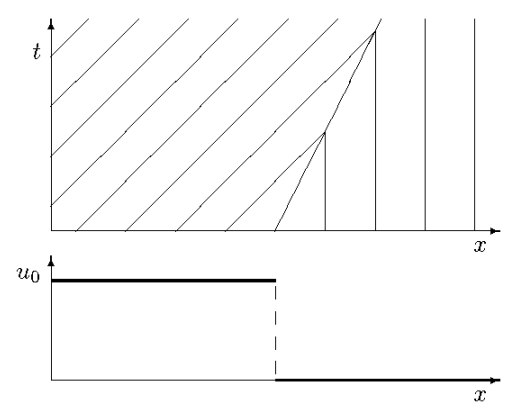
\includegraphics[width=.78\linewidth]{figures/burgers-decreasing-shock-source.png}
\caption{激波解.}\label{fig:burgers-decreasing-shock}
\end{figure}

\subsubsection{多重性}\label{subsec:weak-solution-multiplicity}

再次考虑 Burgers 方程, 但这次采用初始数据
\begin{equation}\label{eq:burgers-increasing-step-data}
u_0(x):=\begin{cases}0,&x<0\\1,&x\geq0.\end{cases}
\end{equation}
这就是 Figure~\ref{fig:characteristic-gap} 中考察的情形, 特征线法留下了一块尚未定义解的空白区域. 应如何填补这块空白? 若寻找一个不连续解, 使其在激波左侧恒为零, 右侧恒为一, 则 Rankine-Hugoniot 条件 \eqref{eq:rankine-hugoniot-jump-condition} 给出
\begin{equation}\label{eq:burgers-increasing-step-shock-speed}
s(0-1)=\dfrac{0^2}{2}-\dfrac{1^2}{2},
\end{equation}
即与先前一样, $s=1/2$. Figure~\ref{fig:burgers-two-weak-solutions} 上方的特征线图展示了这个解.

\PDEIndexMark{idx:burgers-rarefaction-alternative}不过, 还有另一种填补空白并得到解的方法. 以下连续解称为\emph{稀疏波}, 下文 Section~\ref{sec:riemann-problems} 将进一步说明其由来.
\begin{equation}\label{eq:burgers-rarefaction-wave}
u(x,t):=\begin{cases}0,&x<0\\x/t,&0\leq x<t\\1,&t\leq x.\end{cases}
\end{equation}
读者应验证, 任意作为 \eqref{eq:conservation-law-system} 分片经典解的连续函数都是弱解 (参见 Theorem~\ref{thm:rankine-hugoniot} 的证明).

\begin{figure}[H]
\centering
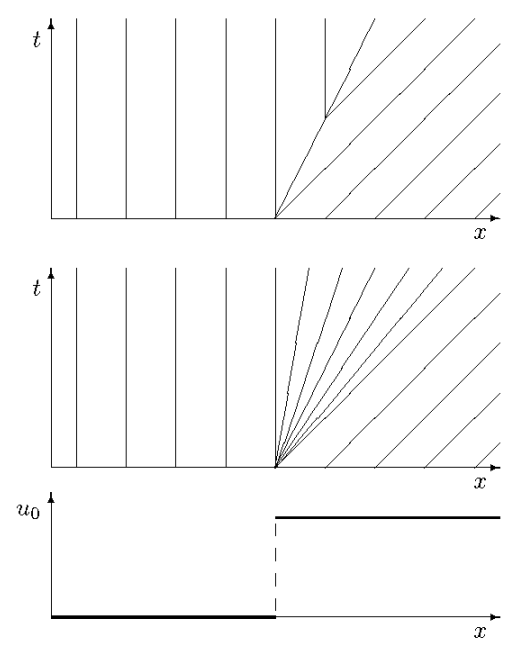
\includegraphics[width=.78\linewidth]{figures/burgers-two-weak-solutions-source.png}
\caption{同一初始数据的两个弱解: 激波 (上) 与稀疏波或"扇形"波 (下).}\label{fig:burgers-two-weak-solutions}
\end{figure}

Figure~\ref{fig:burgers-two-weak-solutions} 下方的特征线图展示了这个解.

事实上, 通过组合激波与稀疏波, 可以构造一整个连续统的解. 对
\begin{equation}\label{eq:burgers-continuum-solution-data}
u_0(x):=\begin{cases}0,&x<0\\1,&x\geq0,\end{cases}
\end{equation}
有以下以 $\gamma\in[0,1]$ 为参数的解族:
\begin{equation}\label{eq:burgers-continuum-weak-solutions}
u_\gamma(x,t):=\begin{cases}0,&-\infty<x\leq0\\x/t,&0<x\leq\gamma t\\\gamma,&\gamma t<x\leq\dfrac{\gamma+1}{2}t\\1,&\dfrac{\gamma+1}{2}t<x<\infty.\end{cases}
\end{equation}
下文 Problem~\ref{ex:sketch-mixed-rarefaction-shock} 要求读者画出这个解的特征线图.

\subsubsection{Lax 激波条件}\label{subsec:lax-shock-condition}

\PDEIndexMark{idx:shock-selection-introduction}如此大量的解的多重性是无法接受的. 与守恒律相关的物理, 尤其是气体动力学这个例子, 使人期待解是唯一的. 因而需要一个"选择准则", 从许多可能的弱解中选出物理上合理的解.

已有多种这样的准则被提出, 但哪一种才是"正确的", 迄今尚无普遍共识. 粗略地说, 对某些"简单"类型的守恒律, 所有条件都一致, 但在一些病态情形下它们并不一致. 不幸的是 (如果打算在这一领域从事研究, 也可以说是幸运的), 某些病态情形出现在重要的物理问题中 (例如石油开采模型), 所以最佳选择准则的问题并非仅仅是数学上的诡辩.

本节介绍的准则是使用最广泛的准则之一, 主要因为它在下文讨论的 Riemann 问题中相当容易实施. Peter Lax 在二十世纪五十年代提出了这一准则~\cite{La}. 将在 Section~\ref{sec:entropy-selection-criteria} 中考察一些与 Lax 条件竞争的准则.

\begin{Definition}{Lax 激波条件}
\label{def:lax-shock-condition}
假设 $\bm{u}$ 是严格双曲守恒律方程组的分片经典解. 假设 $\bm{u}$ 在曲线 $C$ 上有跳跃间断, $\bm{u}^l$ 和 $\bm{u}^r$ 分别是 $\bm{u}$ 在点 $\bm{p}\in C$ 处的左极限值与右极限值 (参见 \eqref{eq:conservation-jump-definition}). 再假设 $C$ 在 $\bm{p}$ 处的斜率为 $s$. 若这一不连续解在每个 $\bm{p}\in C$ 处满足 Rankine-Hugoniot 条件 \eqref{eq:rankine-hugoniot-jump-condition}, 并且存在整数 $k$, 满足 $1\leq k\leq n$, 使得
\begin{equation}\label{eq:lax-shock-condition}
\begin{gathered}
\lambda_1(\bm{u}^l)<\lambda_{k-1}(\bm{u}^l)<s<\lambda_k(\bm{u}^l)<\lambda_n(\bm{u}^l),\\
\lambda_1(\bm{u}^r)<\lambda_k(\bm{u}^r)<s<\lambda_{k+1}(\bm{u}^r)<\lambda_n(\bm{u}^r).
\end{gathered}
\end{equation}
则认为它是容许的, 并称为 \textbf{k-shock}. 因此, 左侧恰有 $k-1$ 个特征速度 $\lambda_j(\bm{u}^l)$ 小于斜率 $s$, 右侧恰有 $n-k$ 个速度 $\lambda_j(\bm{u}^r)$ 大于斜率 $s$.
\end{Definition}

\begin{Example}{单个守恒律}
\label{ex:scalar-lax-shock}
对 Burgers 方程, Lax 激波条件 \eqref{eq:lax-shock-condition} 化为
\begin{equation}\label{eq:burgers-lax-condition}
u^l>s>u^r,
\end{equation}
所以只能跨激波"向下跳跃". 这就排除了 Figure~\ref{fig:burgers-two-weak-solutions} 中所描述的特征线离开间断处的不连续弱解. 更一般地, 对单个守恒律
\[
u_t+f(u)_x=0,
\]
有
\begin{equation}\label{eq:scalar-lax-condition}
f'(u^l)>s>f'(u^r).
\end{equation}
因此, 与 Burgers 方程的情形一样, 对任意单个守恒律, Lax 准则要求特征线汇入激波. 这常被描述为"信息损失", 而且如后文将看到的, Lax 条件与热力学第二定律的某个版本有关.

读者还应注意单个守恒律的凸性与 Lax 激波条件之间的关系 (参见 Problem~\ref{ex:convexity-lax-scalar-shock}).
\end{Example}

\begin{Example}{$p$ 方程组}
\label{ex:p-system-lax-shock}
对 $2\times2$ 方程组, Lax 条件要求 "1-shock" 满足
\begin{equation}\label{eq:two-system-first-shock-condition}
s<\lambda_1(\bm{u}^l),\quad\lambda_1(\bm{u}^r)<s<\lambda_2(\bm{u}^r),
\end{equation}
并要求 "2-shock" 满足
\begin{equation}\label{eq:two-system-second-shock-condition}
\lambda_1(\bm{u}^l)<s<\lambda_2(\bm{u}^l),\quad\lambda_2(\bm{u}^r)<s.
\end{equation}
在 $p$ 方程组的情形下, 有
\begin{equation}\label{eq:p-system-eigenvalue-signs}
\lambda_1=-\sqrt{-p'(w)}<0<\sqrt{-p'(w)}=\lambda_2;
\end{equation}
这表明 1-shock 具有负速度 (常称为"后向激波"), 并满足
\begin{equation}\label{eq:p-system-back-shock-speeds}
-\sqrt{-p'(w^r)}<s<-\sqrt{-p'(w^l)},
\end{equation}
而 2-shock (也称为"前向激波") 具有正速度, 并满足
\begin{equation}\label{eq:p-system-front-shock-speeds}
\sqrt{-p'(w^r)}<s<\sqrt{-p'(w^l)}.
\end{equation}
注意, 若假设 $p''>0$ 以保证真正非线性, 则 $w\mapsto\sqrt{-p'(w)}$ 严格递减. 因此, 此时 1-shock 的条件 \eqref{eq:p-system-back-shock-speeds} 蕴含
\begin{equation}\label{eq:p-system-back-shock-volume-jump}
w^r<w^l,
\end{equation}
而 2-shock 的条件 \eqref{eq:p-system-front-shock-speeds} 蕴含
\begin{equation}\label{eq:p-system-front-shock-volume-jump}
w^l<w^r.
\end{equation}

\end{Example}
